\newpage
\subsection{Hidden Subset}
Analog zu den \textit{Naked Subset}-Techniken ist auch \textit{Hidden Subset} ein Sammelbegriff. Er beinhaltet die Techniken \textit{Hidden Pair}, \textit{Hidden Triple} und \textit{Hidden Quadruple}. Auch hier ändert sich nur die Anzahl der betrachteten Kandidatenlisten. Hier soll exemplarisch die Technik \textit{Hidden Tuple} erklärt werden, im folgenden Beispiel wird dann die Technik \textit{Hidden Quadruple} angewendet.\\
Wenn man in einer Figur zwei Zahlen findet, die ausschließlich in den zwei gleichen Zellen vorkommen können, dann müssen diese beiden Zahlen in die beiden Zellen gesetzt werden. Daher kann man alle anderen Kandidaten in den Zellen von der Kandidatenliste streichen.

\begin{figure}[h]
\begin{center}
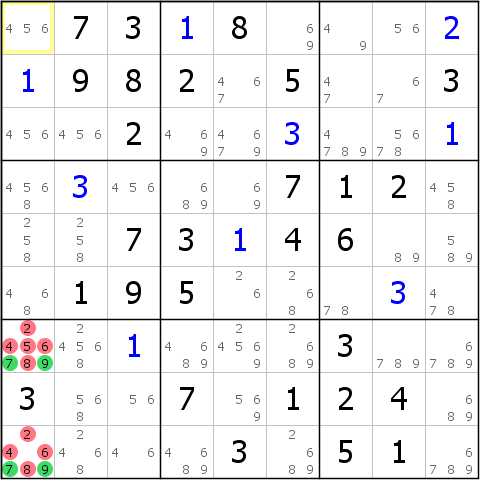
\includegraphics{./img/hidden_subset.png}
\caption{Hidden Subset - Hidden Quadruple}
\end{center}
\end{figure}

In \textbf{Abbildung 3.7} betrachten wir den Block 8 und in diesem Block die Zellen z6s5, z6s6, z7s5 und z7s6. Nur in diesen Zellen können die Zahlen 4, 5, 6 und 8 vorkommen. Da wir diese vier Zahlen nun auf die vier Zellen verteilen müssen gibt es dort keinen Platz mehr für andere Zahlen. Diese können also aus den Kandidatenlisten entfernt werden.
